\documentclass{article}
\usepackage[utf8]{inputenc}
\usepackage[english]{babel}
\usepackage{graphicx}
%\usepackage[font=it]{caption}
\usepackage[textfont=it]{caption}

\usepackage[en-US]{datetime2}
\usepackage{minted}
%\usemintedstyle{solarizedlight}

\usepackage{hyperref}
\usepackage{cleveref}

\title{Milestone 1 Evaluation\\
{\small CSE 232B, UC San Diego, Spring Q 2015}}
\author{Jens Emil Gydesen\thanks{UCSD SID: Ublah} \and
        Martin Bjeldbak Madsen\thanks{UCSD SID: U6616356}}
\date{\DTMdisplaydate{2015}{5}{13}{3}, \DTMdisplaytime{11}{10}{00}}

\begin{document}
\maketitle

Below is our brief report of milestone 2. We did \emph{not} finish the rewriting of the queries. We did, however, implement the join operation in our execution engine and we are also able to produce dependency graphs. 

The repository for this project can be found here: \url{https://github.com/martinbmadsen/xquery-processor}. Although, while the quarter is active, this repository is kept private.

\section{Query 1}

\subsection{Query}\label{sec:query1query}

\begin{listing}[H]
\begin{minted}{xquery}
<acts>{
  for $s in document("j_caesar.xml")//SPEAKER, 
      $a in document("j_caesar.xml")//ACT, 
      $sp in $a//SPEAKER,
      $stxt in $s/text()
  where $sp eq $s and $stxt = "CASCA"
  return <act>{ $a/TITLE/text()} </act>
}</acts>
\end{minted}
\caption{The first query.}\label{lst:query1}
\end{listing}

\subsection{Dependency Graph}
\begin{figure}[H]
  \centering
  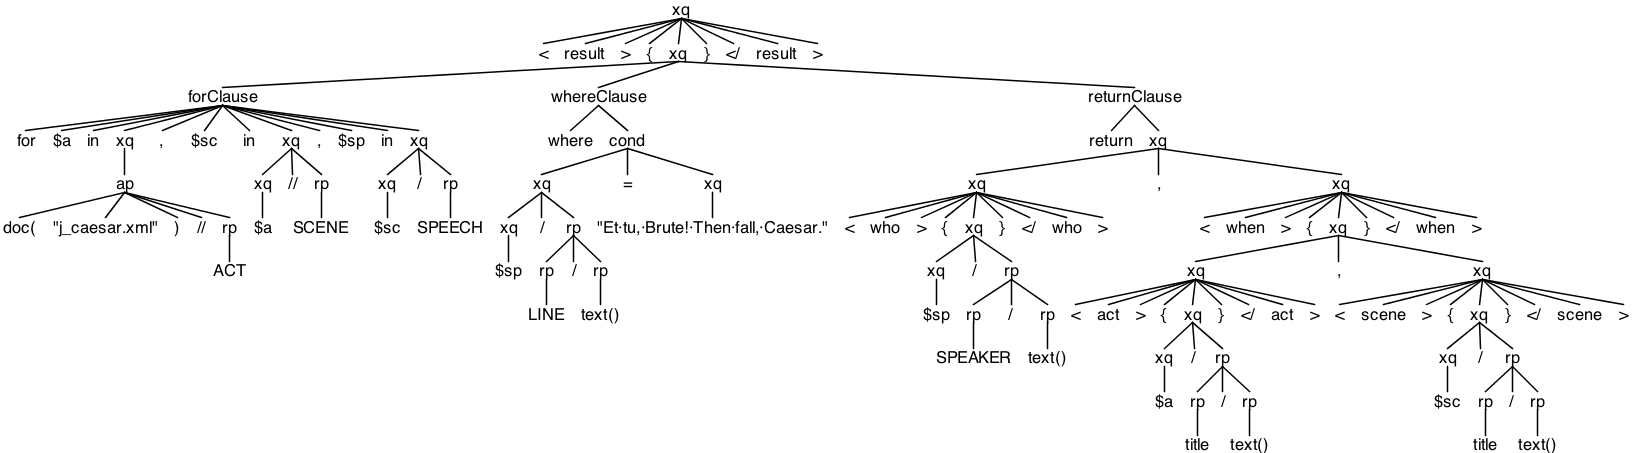
\includegraphics[width=\linewidth]{imgs/antlr4_parse_tree_query_1.png}
  \caption{Parse tree for the first query.}\label{fig:parseTree1}
\end{figure}

\section{Query 2}

\subsection{Query}

\begin{listing}[H]
\begin{minted}{xquery}
for $a1 in document("j_caesar.xml")//ACT,
    $a2 in document("j_caesar.xml")//ACT,
    $a3 in document("j_caesar.xml")//ACT,
    $a4 in document("j_caesar.xml")//ACT,

    $sc1 in $a1//SCENE,
    $sc2 in $a2//SCENE,
    $sc3 in $a3//SCENE,
    $sc4 in $a4//SCENE,

    $sp1 in $sc1//SPEAKER,
    $sp2 in $sc2//SPEAKER,
    $sp3 in $sc3//SPEAKER,
    $sp4 in $sc4//SPEAKER

where $sp1 eq $sp2 and $sp2 eq $sp3 and $sp3 eq $sp4 and $sc1 eq $sc2 and $sc2 eq $sc3 and $sc3 eq $sc4
return <result>{
  <speaker>{$sp1/text()}</speaker>,
  <scene>{$sc1/TITLE/text()}</scene>,
  <act1>{$a1/TITLE/text()}</act1>,
  <act2>{$a2/TITLE/text()}</act2>,
  <act3>{$a3/TITLE/text()}</act3>,
  <act4>{$a4/TITLE/text()}</act4>
}</result>
\end{minted}
\caption{The second query.}\label{lst:query2}
\end{listing}

\subsection{Dependency Graph}
\begin{figure}[H]
  \centering
  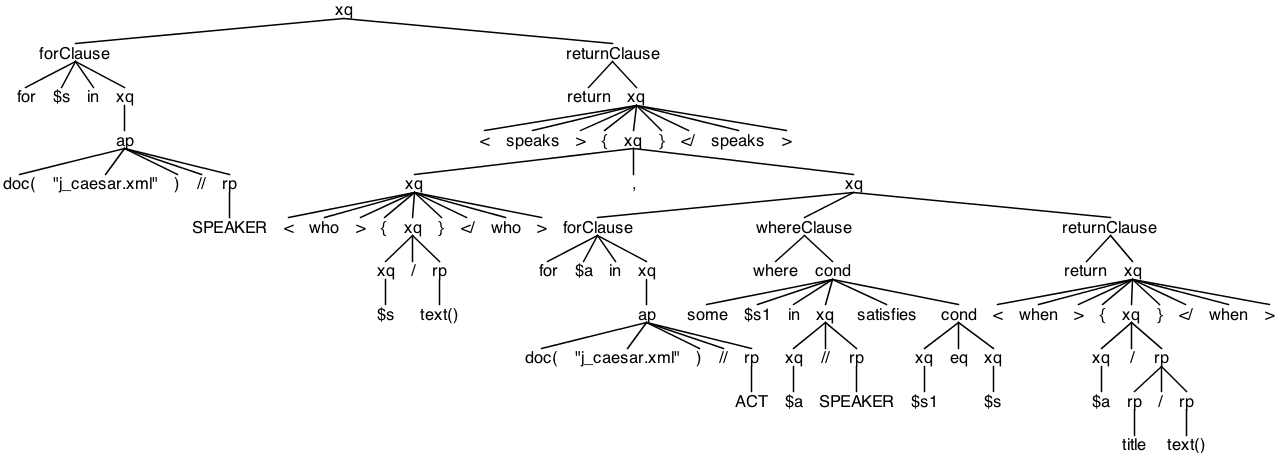
\includegraphics[width=\linewidth]{imgs/antlr4_parse_tree_query_2.png}
  \caption{Parse tree for the second query.}\label{fig:parseTree2}
\end{figure}

\section{Query 3}
\subsection{Query}

\begin{listing}[H]
\begin{minted}{xquery}
for $a in document("j_caesar.xml")//ACT, $at in $a/TITLE/text(),

    $sc1 in $a//SCENE/TITLE,
    $sc2 in $a//SCENE/TITLE,
    $sc3 in $a//SCENE/TITLE,
    $sc4 in $a//SCENE/TITLE,

    $sp1 in $sc1/..//SPEAKER,
    $sp2 in $sc2/..//SPEAKER,
    $sp3 in $sc3/..//SPEAKER,
    $sp4 in $sc4/..//SPEAKER

where $at eq "ACT I" and $sp1 eq $sp2 
      and $sp2 eq $sp3 and $sp3 eq $sp4 
      and $sc1 eq $sc2 and $sc2 eq $sc3 
      and $sc3 eq $sc4
return <result>{
  <speaker>{$sp1/text()}</speaker>,
  <scene>{$sc1/TITLE/text()}</scene>,
  <act>{$a/TITLE/text()}</act>
}</result>
\end{minted}
\caption{The third query.}\label{lst:query3}
\end{listing}

\subsection{Dependency Graph}
\begin{figure}[H]
  \centering
  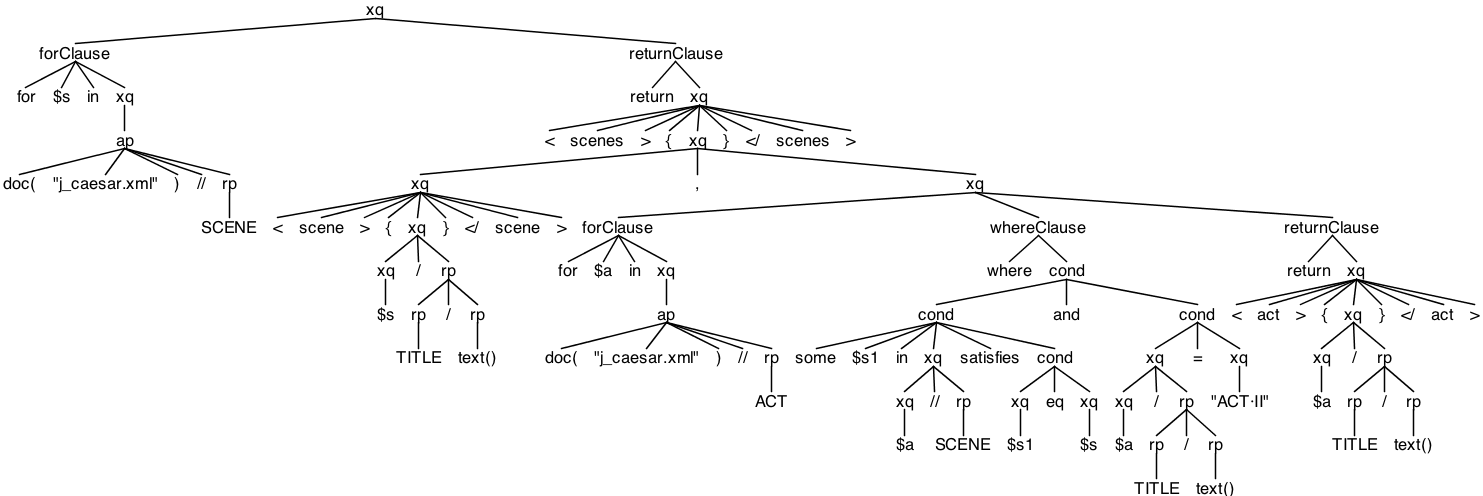
\includegraphics[width=\linewidth]{imgs/antlr4_parse_tree_query_3.png}
  \caption{Parse tree for the third query.}\label{fig:parseTree3}
\end{figure}

\end{document}
